\documentclass{article}
\usepackage[utf8x]{inputenc}
\usepackage{ucs}
\usepackage{amsmath} 
\usepackage{amsfonts}
\usepackage{upgreek}
\usepackage[english,russian]{babel}
\usepackage{graphicx}
\usepackage{float}
\usepackage{textcomp}
\usepackage{hyperref}
\usepackage{geometry}
  \geometry{left=2cm}
  \geometry{right=1.5cm}
  \geometry{top=1cm}
  \geometry{bottom=2cm}
\usepackage{tikz}
\usepackage{ccaption}
\usepackage{multicol}

\usepackage{listings}
%\setlength{\columnsep}{1.5cm}
%\setlength{\columnseprule}{0.2pt}


\begin{document}
\pagenumbering{gobble}

\lstset{
  language=C++,                % choose the language of the code
  basicstyle=\linespread{1.1}\ttfamily,
  columns=fixed,
  fontadjust=true,
  basewidth=0.5em,
  keywordstyle=\color{blue}\bfseries,
  commentstyle=\color{gray},
  stringstyle=\ttfamily\color{orange!50!black},
  showstringspaces=false,
  %numbers=false,                   % where to put the line-numbers
  numbersep=5pt,
  numberstyle=\tiny\color{black},
  numberfirstline=true,
  stepnumber=1,                   % the step between two line-numbers.        
  numbersep=10pt,                  % how far the line-numbers are from the code
  backgroundcolor=\color{white},  % choose the background color. You must add \usepackage{color}
  showstringspaces=false,         % underline spaces within strings
  captionpos=b,                   % sets the caption-position to bottom
  breaklines=true,                % sets automatic line breaking
  breakatwhitespace=true,         % sets if automatic breaks should only happen at whitespace
  xleftmargin=.2in,
  extendedchars=\true,
  keepspaces = true,
}
\lstset{literate=%
   *{0}{{{\color{red!20!violet}0}}}1
    {1}{{{\color{red!20!violet}1}}}1
    {2}{{{\color{red!20!violet}2}}}1
    {3}{{{\color{red!20!violet}3}}}1
    {4}{{{\color{red!20!violet}4}}}1
    {5}{{{\color{red!20!violet}5}}}1
    {6}{{{\color{red!20!violet}6}}}1
    {7}{{{\color{red!20!violet}7}}}1
    {8}{{{\color{red!20!violet}8}}}1
    {9}{{{\color{red!20!violet}9}}}1
}

\title{Семинар \#17: Обработка ошибок. \vspace{-5ex}}\date{}\maketitle

\section*{Часть 1: Классификация ошибок}
Есть множество различных классификаций ошибок, здесь представлена одна из них, которая может отличаться от классификаций в других источниках. Ошибки делятся на:
\begin{itemize}
\item Ошибки времени компиляции
\item Ошибки линковки
\item Ошибки времени выполнения
\item Логические ошибки (ошибки в логике работы программы; могут привести или не привести к ошибке времени выполнения)
\end{itemize}

Под обработкой ошибок обычно понимается обработка ошибок времени выполнения. Их, в свою очередь, можно тоже разделить на 2 части:
\begin{center}
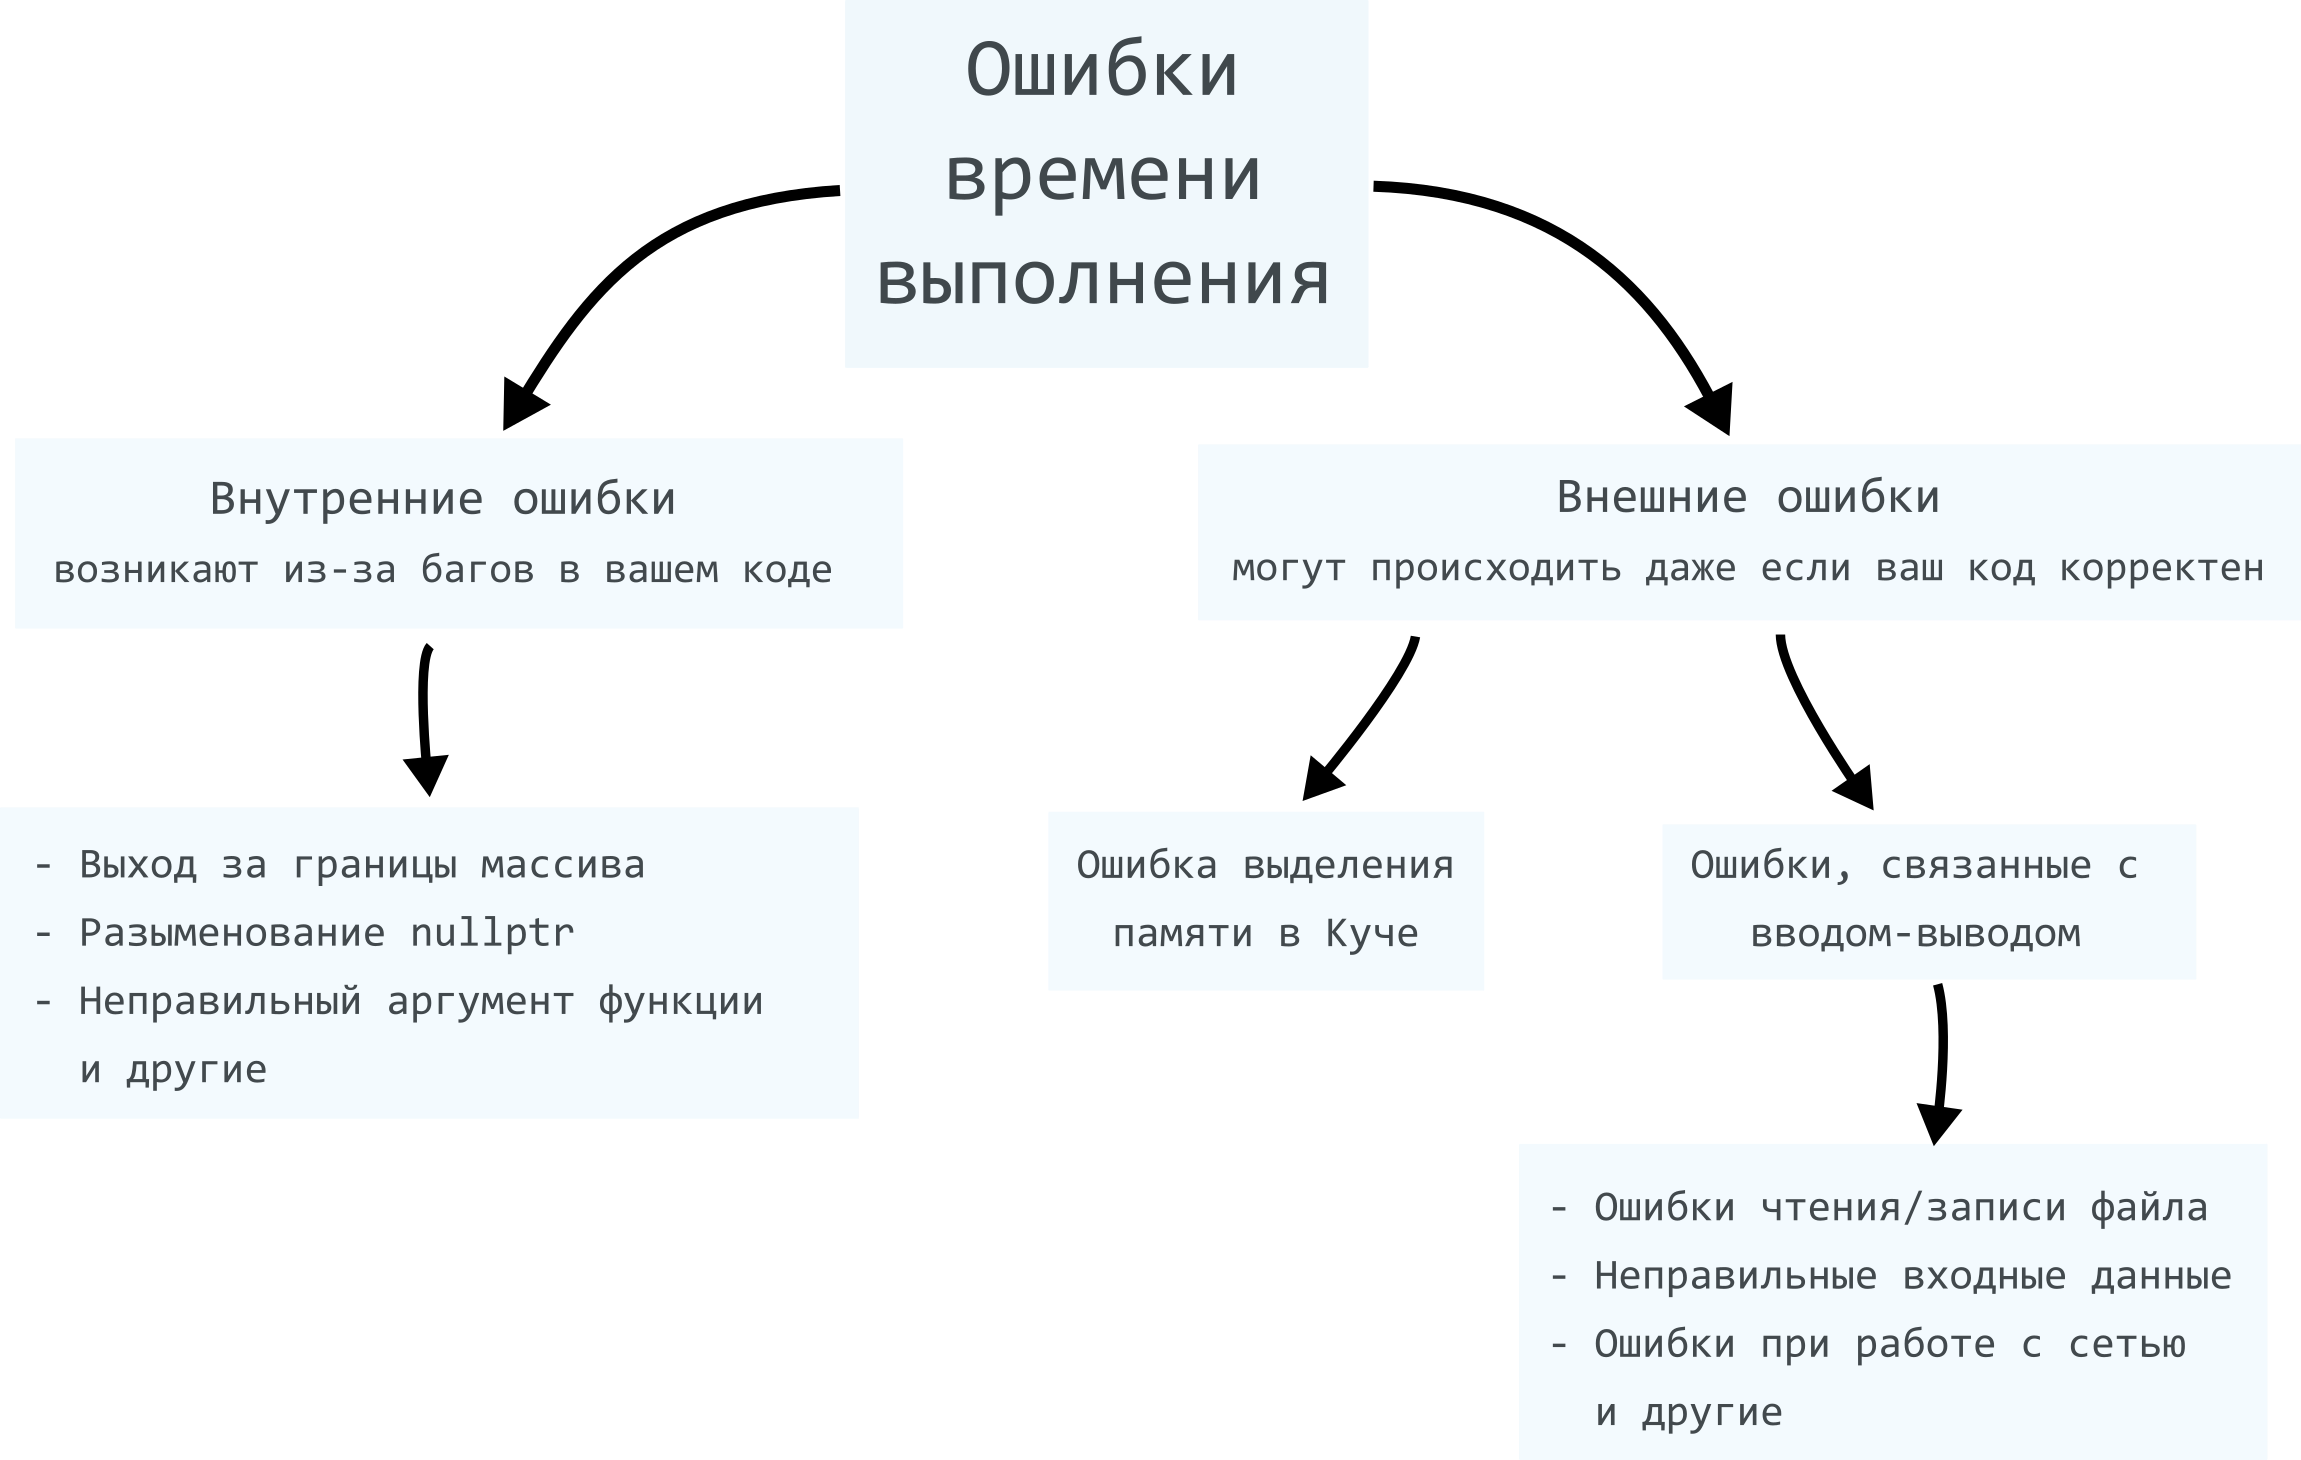
\includegraphics[scale=0.9]{../images/error_types.png}
\end{center}

Эти 2 класса ошибок времени выполнения сильно различаются друг от друга и должны обрабатываться различными способами.

\begin{itemize}
\item От внутренних ошибок, как правило, нельзя востановиться. Лучшее решение в этом случае -- это завершить выполнение программы и вывести сообщение об ошибке.
\item Внешние ошибки часто можно предусмотреть и продумать действия программы при возникновении такой ошибки. Иногда можно даже восстановить работу программы.
\end{itemize}


\newpage
\section*{Часть 2: Методы обработки внутренних ошибок}

\begin{itemize}
\item Ничего не делать
\item \texttt{assert}
\item Контракты (C++26)
\end{itemize}

\begin{lstlisting}
#include <iostream>
#include <cmath>
#include <cassert>
using std::cout, std::endl;

float geometricMean(float a, float b)
{
    assert(a >= 0 && b >= 0);
    return std::sqrt(a * b);
}
int main()
{
    cout << geometricMean(-2, 2) << endl;
}
\end{lstlisting}


\newpage
\section*{Часть 3: Методы обработки внешних ошибок}
\begin{itemize}
\item Использование глабальной переменной
\item Коды возврата
\item Исключения
\end{itemize}


\end{document}